
%% latex JOP_JL_062012.tex

%% bibtex JOP_JL_062012.aux

%% latex JOP_JL_062012.tex

%% dvipdfmx JOP_JL_062012.dvi

%% /usr/share/texmf-texlive/tex/latex/iop
%% dvipdfmx

\documentclass[12pt,twocolumn,iop]{/usr/share/texmf-texlive/tex/latex/iop/iopart}[/usr/share/texmf-texlive/tex/latex/iop/]
\usepackage{graphicx}
\usepackage{ifthen}
\usepackage{dcolumn}% Align table columns on decimal point
\usepackage{bm}% bold math
\usepackage{multirow}
\usepackage{booktabs}
\usepackage{bm}% bold math
\usepackage{amsbsy}
\usepackage{amsmath}
\usepackage{amssymb}
\usepackage{subfigure}
\usepackage{multicol}
\usepackage{citesort}


\newcommand{\two}{\mspace{-2.0mu}}
\newcommand{\four}{\mspace{-4.0mu}}
\newcommand{\plus}{\mspace{-4.5mu}+\mspace{-3.5mu}}
\newcommand{\minus}{\mspace{-4.5mu}-\mspace{-3.5mu}}
\newcommand{\pp}{'\mspace{-2.0mu}'}

\newcommand{\xlb}[4]{#1\ifthenelse{\equal{#2}{0}}{}{_{\alpha #2}}
\mspace{-2.0mu}\genfrac{(}{)}{0pt}{1}{\ifthenelse{\equal{#3}{0}}{0}{l #3}} {\ifthenelse{\equal{#4}{0}}{0}{b #4}}}

\newcommand{\xkv}[4]{#1\mspace{-5.0mu}\left(\mspace{-8.0mu}\begin{smallmatrix}#2\four{}\four{}\mspace{-8.0mu}&\pmb{\kappa}#3\\&\nu #4\end{smallmatrix}\mspace{-5.0mu}\right)}

\newcommand{\evect}[6]{#1\mspace{-4.0mu}\left(\mspace{-8.0mu}\begin{smallmatrix}#2\mspace{-8.0mu}&\pmb{\kappa} #3 &b #5\\&\nu #4 &\alpha #6\end{smallmatrix}\mspace{-5.0mu}\right)}

\newcommand{\varmat}[8]{\mspace{-5.0mu}\left(\mspace{-8.0mu}\begin{smallmatrix}\ifthenelse{\equal{#3}{0}}{\mspace{-8.0mu}&b_{#1}&b_{#2}\\&\alpha_{#1}&\alpha_{#2}} {\ifthenelse{\equal{#7}{0}}{#1\mspace{-8.0mu}&\pmb{\kappa}#2#3\mspace{-8.0mu}&\pmb{\kappa}#4#5\mspace{-8.0mu}&\pmb{\kappa}#6\\&\nu#2&\nu#4&\nu#6} {#1\mspace{-8.0mu}&\pmb{\kappa}#2#3\mspace{-8.0mu}&\pmb{\kappa}#4#5\mspace{-8.0mu}&\pmb{\kappa}#6#7\mspace{-8.0mu}&\pmb{\kappa}#8\\&\nu#2&\nu#4&\nu#6&\nu#8}}\end{smallmatrix}\mspace{-5.0mu}\right)}

\newcommand{\EXP}[1]{\exp\mspace{-5.0mu}\left[#1\right]\mspace{-3.0mu}}

\newcommand{\tpp}[2]{\left(\mspace{-2.0mu}\xkv{\omega}{}{}{}#1\xkv{\omega}{}{'}{'}#2\xkv{\omega}{}{\pp}{\pp}\mspace{-2.0mu}\right)}

\newcommand{\be} {\begin{eqnarray}}
\newcommand{\ee} {\end{eqnarray}}
\newcommand{\f}[2]{\ensuremath{\frac{\displaystyle{#1}}{\displaystyle{#2}}}}
\newcommand{\lr}[1]{\langle{#1}\rangle}

\newcommand{\SUM}[2]{\ifthenelse{\equal{#1}{0}}{\sum_{\alpha_{#2},b_{#2},l_{#2}}^{3,n,N}} {\ifthenelse{\equal{#1}{1}}{\sum_{\alpha_{#2},b_{#2}}^{3,n}}{\sum_{\pmb{\kappa}#2,\nu#2}^{N,3n}}}}

\newcommand{\SUMprime}[2]{\ifthenelse{\equal{#1}{0}}{\sum_{\alpha_{#2},b_{#2},l_{#2}}^{3,n,N}} {\ifthenelse{\equal{#1}{1}}{\sum_{\alpha_{#2},b_{#2}}^{3,n}}{\sum_{\pmb{\kappa}^{'}#2,\nu#2}^{N,3n}}}}

\newcommand{\SUMalpha}[2]{\ifthenelse{\equal{#1}{0}}{\sum_{\alpha_{#2}}^{3}} {\ifthenelse{\equal{#1}{1}}{\sum_{\alpha_{#2},b_{#2}}^{3,n}}{\sum_{\pmb{\kappa}#2,\nu#2}^{N,3n}}}}

\newcommand{\SUMalphap}[2]{\ifthenelse{\equal{#1}{0}}{\sum_{\alpha'_{#2}}^{3}} {\ifthenelse{\equal{#1}{1}}{\sum_{\alpha'_{#2},b'_{#2}}^{3,n}}{\sum_{\pmb{\kappa}#2,\nu#2}^{N,3n}}}}

\newcommand{\SUMb}[2]{\ifthenelse{\equal{#1}{0}}{\sum_{b_{#2}}^{n}} {\ifthenelse{\equal{#1}{1}}{\sum_{\alpha_{#2},b_{#2}}^{3,n}}{\sum_{\pmb{\kappa}#2,\nu#2}^{N,3n}}}}

\newcommand{\SUMbp}[2]{\ifthenelse{\equal{#1}{0}}{\sum_{b'_{#2}}^{n}} {\ifthenelse{\equal{#1}{1}}{\sum_{\alpha'_{#2},b'_{#2}}^{3,n}}{\sum_{\pmb{\kappa}#2,\nu#2}^{N,3n}}}}

\newcommand{\SUMl}[2]{\ifthenelse{\equal{#1}{0}}{\sum_{l_{#2}}^{N}} {\ifthenelse{\equal{#1}{1}}{\sum_{\alpha_{#2},b_{#2}}^{3,n}}{\sum_{\pmb{\kappa}#2,\nu#2}^{N,3n}}}}

\newcommand{\SUMlp}[2]{\ifthenelse{\equal{#1}{0}}{\sum_{l'_{#2}}^{N}} {\ifthenelse{\equal{#1}{1}}{\sum_{\alpha'_{#2},b'_{#2}}^{3,n}}{\sum_{\pmb{\kappa}#2,\nu#2}^{N,3n}}}}

\newcommand{\abcdt}[5]{\mspace{-4.0mu}\left(\mspace{-8.0mu}\begin{smallmatrix}&\ifthenelse{\equal{#1}{}}{a}{#1}&\ifthenelse{\equal{#3}{}}{c}{#3}\\&\ifthenelse{\equal{#2}{}}{b}{#2}&\ifthenelse{\equal{#4}{}}{d}{#4}\end{smallmatrix}\mspace{-2.0mu};\ifthenelse{\equal{#5}{}}{t}{#5}\right)}

\newcommand{\abcd}[4]{\mspace{-4.0mu}\left(\mspace{-8.0mu}\begin{smallmatrix}&\ifthenelse{\equal{#1}{}}{a}{#1}&\ifthenelse{\equal{#3}{}}{c}{#3}\\&\ifthenelse{\equal{#2}{}}{b}{#2}&\ifthenelse{\equal{#4}{}}{d}{#4}\end{smallmatrix}\mspace{-3.0mu}\right)}

\newcommand{\abt}[3]{\mspace{-4.0mu}\left(\mspace{-8.0mu}\begin{smallmatrix}&\ifthenelse{\equal{#1}{}}{a}{#1} \\&\ifthenelse{\equal{#2}{}}{b}{#2}\end{smallmatrix}\mspace{-2.0mu};\ifthenelse{\equal{#3}{}}{t}{#3}\right)}

\newcommand{\ab}[2]{\mspace{-4.0mu}\left(\mspace{-8.0mu}\begin{smallmatrix}&\ifthenelse{\equal{#1}{}}{a}{#1} \\&\ifthenelse{\equal{#2}{}}{b}{#2}\end{smallmatrix}\mspace{-3.0mu}\right)}

\newcommand{\kvbat}{\mspace{-4.0mu}\left(\mspace{-8.0mu}\begin{smallmatrix} &\pmb{\kappa} &b \\ &\nu &\alpha\end{smallmatrix}\mspace{-2.0mu};t\right)}

\newcommand{\kvbatp}{\mspace{-4.0mu}\left(\mspace{-8.0mu}\begin{smallmatrix} &\pmb{\kappa} &b' \\ &\nu &\alpha'\end{smallmatrix}\mspace{-2.0mu};t\right)}

\newcommand{\kvbaw}{\mspace{-4.0mu}\left(\mspace{-8.0mu}\begin{smallmatrix} &\pmb{\kappa} &b \\ &\nu &\alpha\end{smallmatrix}\mspace{-2.0mu};\omega\right)}

\newcommand{\kvbawp}{\mspace{-4.0mu}\left(\mspace{-8.0mu}\begin{smallmatrix} &\pmb{\kappa} &b' \\ &\nu &\alpha'\end{smallmatrix}\mspace{-2.0mu};\omega\right)}

\newcommand{\kvba}{\mspace{-4.0mu}\left(\mspace{-8.0mu}\begin{smallmatrix} &\pmb{\kappa} &b \\ &\nu &\alpha\end{smallmatrix}\mspace{-3.0mu}\right)}

\newcommand{\kvbap}{\mspace{-4.0mu}\left(\mspace{-8.0mu}\begin{smallmatrix} &\pmb{\kappa} &b' \\ &\nu &\alpha'\end{smallmatrix}\mspace{-3.0mu}\right)}

\newcommand{\kpvba}{\mspace{-4.0mu}\left(\mspace{-8.0mu}\begin{smallmatrix} &\pmb{\kappa}^{'} &b \\ &\nu &\alpha\end{smallmatrix}\mspace{-3.0mu}\right)}

\newcommand{\kva}{\mspace{-4.0mu}\left(\mspace{-8.0mu}\begin{smallmatrix} &\pmb{\kappa} \\ &\nu &\alpha\end{smallmatrix}\mspace{-3.0mu}\right)}

\newcommand{\kvap}{\mspace{-4.0mu}\left(\mspace{-8.0mu}\begin{smallmatrix} &\pmb{\kappa} \\ &\nu &\alpha'\end{smallmatrix}\mspace{-3.0mu}\right)}

\newcommand{\kvb}{\mspace{-4.0mu}\left(\mspace{-8.0mu}\begin{smallmatrix} &\pmb{\kappa} &b \\ &\nu \end{smallmatrix}\mspace{-3.0mu}\right)}

\newcommand{\kvbp}{\mspace{-4.0mu}\left(\mspace{-8.0mu}\begin{smallmatrix} &\pmb{\kappa} &b' \\ &\nu \end{smallmatrix}\mspace{-3.0mu}\right)}

\newcommand{\kvt}{\mspace{-4.0mu}\left(\mspace{-8.0mu}\begin{smallmatrix}&\pmb{\kappa} \\&\nu\end{smallmatrix}\mspace{-2.0mu};t\right)}

\newcommand{\kpvt}{\mspace{-4.0mu}\left(\mspace{-8.0mu}\begin{smallmatrix}&\pmb{\kappa}^{'} \\&\nu\end{smallmatrix}\mspace{-2.0mu};t\right)}

\newcommand{\kvw}{\mspace{-4.0mu}\left(\mspace{-8.0mu}\begin{smallmatrix}&\pmb{\kappa} \\&\nu\end{smallmatrix}\mspace{-2.0mu};\omega\right)}

\newcommand{\kv}{\mspace{-4.0mu}\left(\mspace{-8.0mu}\begin{smallmatrix}&\pmb{\kappa} \\&\nu\end{smallmatrix}\mspace{-3.0mu}\right)}

\newcommand{\lbt}{\mspace{-4.0mu}\left(\mspace{-8.0mu}\begin{smallmatrix}&l \\&b\end{smallmatrix}\mspace{-2.0mu};t\right)}

\newcommand{\lbtp}{\mspace{-4.0mu}\left(\mspace{-8.0mu}\begin{smallmatrix}&l' \\&b'\end{smallmatrix}\mspace{-2.0mu};t\right)}

\newcommand{\lt}{\mspace{-4.0mu}\left(\mspace{-8.0mu}\begin{smallmatrix}&l\end{smallmatrix}\mspace{-2.0mu};t\right)}

\newcommand{\ltp}{\mspace{-4.0mu}\left(\mspace{-8.0mu}\begin{smallmatrix}&l'\end{smallmatrix}\mspace{-2.0mu};t\right)}

\newcommand{\lb}{\mspace{-4.0mu}\left(\mspace{-8.0mu}\begin{smallmatrix}&l \\&b\end{smallmatrix}\mspace{-3.0mu}\right)}

\newcommand{\lbp}{\mspace{-4.0mu}\left(\mspace{-8.0mu}\begin{smallmatrix}&l' \\&b'\end{smallmatrix}\mspace{-3.0mu}\right)}


%---------------------------------------------------------------------------------------------

\begin{document}

\title{Comparison and evaluation of spectral energy methods for predicting phonon properties}

\author{J M Larkin$^1$, J E Turney$^1$,
A D Massicotte$^1$, C H Amon$^{1,2}$  and A J H McGaughey$^1$ \ead{mcgaughey@cmu.edu}}

\address{$^1$ Department of Mechanical Engineering\\Carnegie Mellon University\\Pittsburgh, PA 15213}
\address{$^2$ Department of Mechanical \& Industrial Engineering, University of Toronto, Toronto, Ontario, Canada M5S 3G8}


\date{\today}

\begin{abstract}
Two frequency-domain methods for predicting phonon frequencies and lifetimes
using the phonon spectral energy density are described. Both methods draw
input from molecular dynamics simulations and lattice dynamics calculations,
but differ in the form of the phonon spectral energy density.
One phonon spectral energy density expression (referred to as $\Phi$) can be
formally derived from lattice dynamics theory. A similar approach in the
time domain has been validated [Turney et al. \emph{Phys. Rev. B} \textbf{79}, 224305
(2009)]. The other phonon spectral energy density expression (referred to as
$\Phi'$) has been proposed [Thomas et al., \emph{Phys. Rev. B} \textbf{81}, 081411(R) (2010)]
but not validated. The expressions for $\Phi$ and $\Phi'$ are presented and then
applied to predict the phonon properties and thermal conductivities of three
systems: Lennard-Jones argon, Stillinger-Weber silicon, and a carbon
nanotube modeled using the Reactive Empirical Bond Order potential. $\Phi'$ does not capture the total
phonon spectral energy density predicted by $\Phi$ and therefore cannot
correctly predict the phonon lifetimes or thermal conductivity. Its use in
future work is discouraged.
\end{abstract}

\pacs{63.20-e,63.20.D-,63.20.K-,63.20.kg}

\submitto{\JPCM}

\maketitle

%\begin{multicols}{2}

\section{\label{Section_Introduction}Introduction}

Phonons are the dominant carriers of thermal energy in dielectric
and semiconducting crystals \cite{cahill2003,goodson2005,srivastava1990,wallace1972,maradudin1974,dove1993}. While
substantial effort has been devoted to developing theories of phonon
transport, the current understanding is incomplete, even in bulk materials. For
example, which phonon modes dominate thermal energy transport and the importance of
interactions involving four or more phonons are still being investigated \cite{wallace1972,srivastava1990,broido2007,esfarjani2011,cahill2003}.  The
situation becomes more complicated in nanostructures, where the phonons also interact with free surfaces and interfaces \cite{asheghi1997,balandin1997,li1997,tian2011,Hochbaum2011,Martin2011,Yu2011,Hopkins2011,landry2008,mcgaughey2011a,landry2009,landry2009b,landry2010}.

Analytical models of thermal transport, such as the Debye model, are limited by
the necessary approximations and assumptions \cite{callaway1959,holland1963,mcgaughey2011a}. With the Green-Kubo or
non-equilibrium direct methods, molecular dynamics (MD) simulations can be used to predict thermal
conductivity, but only in a classical (i.e., high-temperature) framework \cite{ladd1986,mcgaughey2004c,landry2008,schelling2002,sellan2010a,esfarjani2011,turney2009a}. Because the analysis in these two MD-based methods is performed at the system level, no information about the phonons is obtained. Phonon specific heats, group velocities, and lifetimes are the required inputs for predicting thermal conductivity at the phonon-mode-level using  Boltzmann transport equation-based models \cite{ladd1986,mcgaughey2004c,mcgaughey2011a,sellan2010b,esfarjani2011,turney2009a,He2011}.
These phonon properties can be predicted using harmonic and anharmonic lattice dynamics
calculations,\cite{maradudin1962,wallace1972,ladd1986,dove1993,turney2009a,turney2009b} where quantum statistical effects can be naturally included. Anharmonic lattice dynamics calculations are limited to three-phonon scattering events, however, and are thus only valid at low temperatures \cite{turney2009a,esfarjani2011,wallace1972,srivastava1990}.

At high temperature, four-phonon and higher-order processes become important to thermal transport \cite{wallace1972,srivastava1990,turney2009a,esfarjani2011}. All orders of phonon processes are present in a MD simulation as the positions and momenta of the atoms are evolved using the full anharmonicity of the interatomic interactions \cite{mcgaughey2004c,esfarjani2011}. Phonon properties can be predicted from a MD simulation using normal mode analysis in the time domain \cite{ladd1986,mcgaughey2004c,henry2008,turney2009a,goicochea2010,He2011}. In Section \ref{S:Subsection_NMD}, we will describe how this approach can be performed in the frequency-domain using the phonon spectral energy density (SED, referred to as $\Phi$). An alternative expression for the phonon SED (referred to herein as $\Phi'$), was recently proposed but has not been rigorously tested \cite{maruyama2003,shiomi2006,thomas2010c}. $\Phi^{'}$ was first used to predict the phonon dispersion curves of carbon nanotubes (CNTs) \cite{maruyama2003}. Thomas et al. used $\Phi'$ to predict the phonon lifetimes and thermal conductivity of isolated and water-filled CNTs, obtaining good agreement with other atomistic predictions \cite{thomas2010c}. The phonon lifetime reductions speculated for water-filled CNTs\cite{thomas2010c} and CNTs on SiO$_2$ substrates\cite{shiomi2011b} suggest that $\Phi'$ captures phonon physics at least qualitatively. The phonon lifetimes and thermal conductivity for PbTe\cite{qiu2011} and Half Heusler alloys\cite{shiomi2011a} have also been predicted using $\Phi'$. De Koker predicted the phonon lifetimes and thermal conductivity for MgO using an expression similar to $\Phi'$ (but different than $\Phi$) \cite{dekoker2009}. Another recent atomistic study using Stillinger-Weber silicon predicted phonon lifetimes using both $\Phi$ and $\Phi'$, but a detailed comparison of the predictions between the two was not performed \cite{Hori2012}.

The objective of this work is to assess the validity of $\Phi'$ as a phonon SED by comparing the phonon properties it predicts to those predicted by $\Phi$. In Section \ref{S:Subsection_NMD}, we derive the correct phonon SED ($\Phi$) from lattice dynamics theory, which requires the phonon mode eigenvectors. The expression for $\Phi$ is well-defined theoretically and has been tested and validated in previous studies in the time domain \cite{ladd1986,turney2009a}. In Section \ref{S:Subsection_Proposed_SED}, we present the proposed alternative expression for the phonon SED, $\Phi'$, which does not require the phonon mode eigenvector \cite{thomas2010c}. Phonon frequencies, lifetimes, and thermal conductivities are then predicted and compared using $\Phi$ and $\Phi'$ for three test systems: Lennard-Jones (LJ) argon\cite{ashcroft1976} in Section \ref{S:Subsection_prop_LJ}, Stillinger-Weber (SW) silicon\cite{stillinger1985} in Section \ref{S:Subsection_prop_SW}, and an (8,8) CNT modeled with the reactive empirical bond order (REBO) potential\cite{brenner2002} in Section \ref{S:Subsection_prop_CNT}. While $\Phi'$ is found to accurately predict the phonon frequencies, we find that it does not correctly predict the phonon lifetimes because it does not capture the total phonon spectral energy density.

\section{\label{S:Section_NMD}Phonon Spectral Energy Density}

\subsection{\label{S:Subsection_NMD}As Derived from Normal Mode Coordinates, $\Phi$}

To derive the correct expression for the phonon SED, $\Phi$, we begin with harmonic lattice dynamics theory \cite{wallace1972,dove1993}. The derivation outlined here is presented in detail in \ref{Appendix_A}.

In reciprocal space, the system Hamiltonian, $H$, is
\begin{equation}\label{E:H_HLD}
\begin{split}
H=&\frac{1}{2}\SUM{}{}\left[\dot{q}^*\kvt \dot{q}\kvt + \omega_0^2\kv q^*\kvt q\kvt\right]\\
 =&\SUM{}{}\left[T\kvt + V\kvt\right],
 \end{split}
\end{equation}
where $t$ is time, $\omega_0\kv$ is the frequency of the phonon mode denoted by
wave vector $\pmb{\kappa}$ and dispersion branch $\nu$, and $N$ and $n$ are
the total number of unit cells and the number of atoms in the unit cell.  The
Hamiltonian is the total system energy and is the sum of the mode- and
time-dependent kinetic and potential energies, $T\kvt$ and $V\kvt$.  The
phonon normal mode coordinate, $q\kvt$ and its time derivative, $\dot{q}\kvt$, are given by
\begin{equation}\label{E:q_HLD}
\begin{split}
q\kvt=&\SUM{0}{}\sqrt{\frac{m_b}{N}}u_{\alpha}\lbt e^*\kvba\EXP{i\pmb{\kappa}\cdot\mathbf{r}_0\ab{l}{0}}
\end{split}
\end{equation}
and
\begin{equation}\label{E:qdot_HLD}
\begin{split}
\dot{q}\kvt{}{}{}=&\SUM{0}{}\sqrt{\frac{m_b}{N}}\dot{u}_{\alpha}\lbt e^*\kvba\EXP{i\pmb{\kappa}\cdot\mathbf{r}_0\ab{l}{0}},
\end{split}
\end{equation}
where $m_b$ is the mass of the $b^{\textrm{th}}$ atom in the unit cell and
$\mathbf{r}_0\ab{l}{0}$ is the equilibrium position vector of the
$l^{\textrm{th}}$ unit cell. The $\alpha$-component of the displacement from
equilibrium, $u_{\alpha}\lbt$, and velocity, $\dot{u}_{\alpha}\lbt$, of the
$b^{\textrm{th}}$ atom in the $l^{\textrm{th}}$ unit cell are time-dependent
and are related to the phonon mode coordinates through the time-independent
eigenvector that has components $e\kvba$.

The expectation value of the kinetic energy of each normal mode in the time domain is
\begin{equation}\label{A:E:ave_T_t}
\begin{split}
\langle T\kv \rangle=&\lim_{\tau_0\rightarrow\infty}\frac{1}{2\tau_0}\int_{0}^{\tau_0}\dot{q}^*\kvt\dot{q}\kvt dt.
\end{split}
\end{equation}
The expectation value of the kinetic energy of the normal mode can be transformed from the time domain to the
frequency domain by Parseval's theorem,\cite{rudin1987}
\begin{equation}\label{E:ave_T_w1}
\begin{split}
T\kvw=&\lim_{\tau_0\rightarrow\infty}\frac{1}{2\tau_0}\left|\frac{1}{\sqrt{2\pi}}\int_{0}^{\tau_0}\dot{q}\kvt\exp(-i\omega t)dt\right|^2.
\end{split}
\end{equation}
Starting from Eq$.$ \eqref{E:ave_T_w1} and following the derivation in \ref{Appendix_A}, one arrives at the expression for the SED of a single phonon mode,
\begin{equation}\label{E:Lorentzian_NMD_2}
\begin{split}
T\kvw = \frac{C_0\kv}{2}\frac{\Gamma\kv/\pi}{[\omega_0\kv-\omega]^2+\Gamma^2\kv},
\end{split}
\end{equation}
which is a Lorentzian function with center at $\omega_0\kv$ and a half-width at half-maximum (linewidth) of
$\Gamma\kv$. The constant $C_0\kv$ is defined in Eq$.$ \eqref{A:E:C_0} in \ref{Appendix_A}. We know from anharmonic lattice dynamics theory that the phonon linewidth is related to the phonon lifetime, $\tau\kv$, by\cite{maradudin1962,ladd1986}
\begin{equation}\label{E:lifetime}
\begin{split}
\tau\kv=&\frac{1}{2\Gamma\kv}.
\end{split}
\end{equation}
The MD simulations we perform here are classical. For a classical system in the harmonic limit (i.e., temperature approaching zero) there is an equipartition of energy and $\sum_{\nu}^{3n} \langle T\kvw \rangle = \sum_{\nu}^{3n} \langle V\kvw \rangle$ \cite{mcquarrie2000}. In an anharmonic system (i.e., a MD simulation), the assumption of equipartition of energy can be tested by predicting the system-level specific heat (see Section \ref{Subsection_Comp_Details_3}). By assuming equipartition of energy, the phonon SED at a particular wavevector is
\begin{equation}\label{E:Lorentzian_NMD}
\begin{split}
\Phi(\pmb{\kappa},\omega) = 2\sum_{\nu}^{3n} T\kvw =& \sum_{\nu}^{3n}C_0\kv\frac{\Gamma\kv/\pi}{[\omega_0\kv-\omega]^2+\Gamma^2\kv},
\end{split}
\end{equation}
which is a superposition of $3n$ Lorentzian functions with centers at $\omega_0\kv$ (one for each polarization). For simplicity, we refer to $\Phi(\pmb{\kappa},\omega)$ as $\Phi$. Given a set of atomic velocities, $\Phi$ can be calculated using Eq$.$ \eqref{E:qdot_HLD} and \eqref{E:ave_T_w1}, and then fit using Eq$.$ \eqref{E:Lorentzian_NMD} to extract the phonon properties $\omega_0\kv$ and $\tau\kv$.

Previous work using normal mode analysis has represented the phonon energy in the time domain,\cite{ladd1986,mcgaughey2004c,henry2008,turney2009a,goicochea2010,He2011} while $\Phi$ is a representation of the phonon energy in the frequency domain. The time- and frequency-domain approaches are mathematically equivalent by use of the Wiener-Khinchin theorem \cite{rudin1987,shiomi2011b}. The frequency-domain approach has the advantage of predicting both the phonon lifetime and frequency by fitting a simpler function than required in the time-domain approach.

\subsection{\label{S:Subsection_Proposed_SED}Alternative Formulation, $\Phi'$}

Now that the phonon SED, $\Phi$, has been properly derived, we seek to motivate the expression $\Phi'$ that was proposed in previous studies but has not been validated \cite{maruyama2003,shiomi2006,thomas2010c}. Thomas et al. \cite{thomas2010c} define
\begin{equation}\label{Lorentzian_SED}
\begin{split}
\Phi'(\pmb{\kappa},\omega) =& \frac{1}{4\pi\tau_0} \sum_\alpha^3 \sum_b^n \frac{m_b}{N}\left| \sum_l^N  \int_{0}^{\tau_0} \dot{u}_{\alpha}\lbt \EXP{\Theta} dt \right|^2,
\end{split}
\end{equation}
where $\Theta \equiv i[\pmb{\kappa}\cdot\mathbf{r}_0\ab{l}{0}-\omega t]$. To understand this expression, we start with the real-space atomic velocities as
represented by the normal mode coordinates,\cite{dove1993}
\begin{equation}\label{E:udot_HLD}
\begin{split}
\dot{u}_{\alpha}\lbt = &\SUMprime{2}{} \frac{1}{\sqrt{m_bN}} \EXP{i\pmb{\kappa}^{'}\cdot\mathbf{r}_0\ab{l}{0}} e^*\kpvba \dot{q}\kpvt{}{}{}.
\end{split}
\end{equation}
Fourier transforming both sides of Eq$.$ \eqref{E:udot_HLD} in time and space, taking the complex modulus, and summing over the atoms in the unit cell and the Cartesian directions yields
\begin{multline}\label{SED}
\lim_{\tau_0\rightarrow\infty}\frac{1}{4\pi\tau_0} \sum_\alpha^3 \sum_b^n \frac{m_b}{N} \left\lvert \sum_l^N  \int_{0}^{\tau_0} \dot{u}_{\alpha}\lbt \EXP{\Theta} dt \right\rvert^2 =
\\ \lim_{\tau_0\rightarrow\infty}\frac{1}{4\pi\tau_0} \sum_\alpha^3 \sum_b^n \left\lvert \frac{m_b^{3/2}}{\sqrt{N}} \sum_l^N \sum_{\nu}^{3n} e^*\kvba \int_{0}^{\tau_0}\dot{q}\kvt\EXP{\Theta}dt \right\rvert^2 ,
\end{multline}
where the the sum over $\pmb{\kappa}^{'}$ on the right-hand-side is reduced to a single wavevector by the orthogonality of the allowed wavevectors over the periodic domain. The expression $\Phi'(\pmb{\kappa},\omega)$ given by Thomas et al. \cite{thomas2010c} (Eq$.$ \eqref{Lorentzian_SED}) is the finite integration of the left-hand-side of Eq$.$ \eqref{SED}. For simplicity, we refer to $\Phi'(\pmb{\kappa},\omega)$ as $\Phi'$. Given a set of atomic velocities, Thomas et al. extract the phonon properties $\omega_0\kv$ and $\tau\kv$ from Eq$.$ \eqref{Lorentzian_SED} by fitting $\Phi'$ for a given wavevector to a superposition of Lorentzian functions.

Thomas et al. \cite{thomas2010c} claim that $\Phi'$ represents the phonon SED. As seen in Eq$.$ \eqref{E:qdot_HLD}, the phonon mode eigenvectors are necessary to properly map the atomic velocities onto the normal mode coordinates. This need for the eigenvectors is the essential difference between the expressions for $\Phi$ and $\Phi'$. The potential advantage of $\Phi'$ is that other than the wavevectors, which can be determined from the crystal structure, no phonon properties need to be known {\em a priori}. However, to identify the degenerate modes in $\Phi'$, the phonon frequencies are necessary (Section \ref{Subsection_Comp_Details_2}). Since $\Phi'$ does not require the phonon mode eigenvector, it can (in principle) be used to study disordered systems or perturbed crystalline systems (e.g. dilute alloys,\cite{shiomi2011a} water-filled CNTs,\cite{thomas2010c} and CNTs on substrates\cite{shiomi2011b}). Despite its use in previous studies, $\Phi'$ has not been rigorously validated.

\section{\label{Section_Comp}Computational Details}

\subsection{\label{Subsection_Comp_Details_1}Allowed Wavevectors}

Now that we have derived and defined the two expressions for the phonon SED, we will provide the computational details of how they can be evaluated and used to predict phonon properties. The SED is defined for the allowed wavevectors of a crystal, which can be specified from the crystal structure's Bravais lattice, its basis (i.e., unit cell), and the size of the computational domain. A $D$-dimensional Bravais lattice is a collection of points with
positions
\begin{equation}\label{crys_pos}
\begin{split}
\mathbf{r}_0\ab{l}{0} =& \sum^D_{\alpha} N_{\alpha}\mathbf{a}_{\alpha},
\end{split}
\end{equation}
where $\mathbf{a}_{\alpha}$ are the lattice vectors and $N_{\alpha}$ is an integer \cite{dove1993}. The unit cell is the building block of the crystal and is placed on the points defined by the Bravais lattice. The equilibrium position of any atom in the crystal can be described by
\begin{equation}\label{crys_pos2}
\begin{split}
\mathbf{r}_0\ab{l}{b} = \mathbf{r}_0\ab{l}{0} + \mathbf{r}_0\ab{0}{b},
\end{split}
\end{equation}
where $\mathbf{r}_0\ab{0}{b}$ is the equilibrium position of the $b^{\textrm{th}}$ atom in the unit cell relative to $\mathbf{r}_0\ab{l}{0}$. The allowed wavevectors for any crystal structure are defined by
\begin{equation}\label{crys_pos3}
\begin{split}
\pmb{\kappa} = \sum_{\alpha} \mathbf{b}_{\alpha} \frac{n_{\alpha}}{N_{\alpha}},
\end{split}
\end{equation}
where $\mathbf{b}_{\alpha}$ are the reciprocal lattice vectors and $-N_{\alpha}/2 < n_{\alpha} \leq N_{\alpha}/2$, where $n_{\alpha}$ are integers and $N_{\alpha}$ are now constant even integers. The wavevectors are taken to be in the first Brillouin zone \cite{ashcroft1976}.

For the LJ argon and SW silicon systems studied here, the cubic conventional cells are used with four (argon) and eight (silicon) atoms per unit cell. For the MD simulations of LJ argon and SW silicon, cubic simulation domains are used (i.e., $N_1 = N_2 = N_3 = N_0$) \cite{mcgaughey2004c,turney2009a,sellan2010a}. For the CNT, the Brillouin zone is one-dimensional, so that $N_1 = N_2 = 1$, and we take $N_3=50$ \cite{thomas2010c}.

\subsection{\label{Subsection_Comp_Details_2}Phonon Lifetimes and Frequencies}

Once the allowed wavevectors are specified, the atomic velocities from an MD simulation can be used to calculate $\Phi'$ using Eq$.$ \eqref{Lorentzian_SED}. To calculate $\Phi$ [Eq$.$ \eqref{E:Lorentzian_NMD}], Eq$.$ \eqref{E:qdot_HLD} and \eqref{E:ave_T_w1} require the phonon mode eigenvector, which can be obtained using lattice dynamics calculations and the finite temperature lattice constant (i.e., quasi-harmonic lattice dynamics calculations) \cite{dove1993}.

The phonon frequencies and lifetimes are found by fitting the spectral curves $\Phi$ and $\Phi'$ with Lorentzian functions using a non-linear least squares method. Both of these phonon properties are independent of the Lorentzian peak magnitude. For $\Phi'$, the different polarizations at a given wavevector are superimposed by definition of Eq$.$ \eqref{Lorentzian_SED}. The different polarizations can be fit individually using single Lorentzian peaks or as a superposition of peaks. At high temperatures, the broadening of the peaks from different polarizations can make it difficult to uniquely locate the peaks in $\Phi'$. Knowledge of the quasi-harmonic frequencies is necessary to identify the unique peaks in $\Phi'$ as well as degeneracies \cite{mcgaughey2006b,turney2009a}.

$\Phi$ has the advantage that degenerate and nearly degenerate polarizations can be isolated and fit individually. The uncertainty in the predicted phonon frequencies is on the order of the frequency resolution used to perform the fast Fourier transforms required to evaluate $\Phi$ and $\Phi'$, which is $10^2-10^4$ less than the phonon frequencies studied in this work (see Sections \ref{S:Subsection_prop_LJ}, \ref{S:Subsection_prop_SW}, and \ref{S:Subsection_prop_CNT}). At the temperatures studied in this work, we find that fitting single or simultaneous peaks in either $\Phi$ or $\Phi'$ results in less than five percent difference in the predicted lifetimes. The uncertainty from fitting the Lorentzian functions is between five and ten percent of the predicted lifetimes, with the error increasing with increasing temperature.\footnote[1]{The range of data must be selected when fitting the Lorentzian functions to $\Phi$ or $\Phi'$. This range should be large enough for the Lorentzian functions to decrease significantly from their value at
half-width at half-maximum, where the linewidth is specified, but not too large as to pick up noise. The error in predicting the lifetime is obtained by varying the range of data
used to fit the Lorentzian function.}

To illustrate the procedure, $\Phi$ was calculated for LJ argon (Section \ref{S:Subsection_prop_LJ}) with $N_0=8$ and $T=20$ K, where $T$ is temperature. $\Phi$ for the three modes of lowest frequency and wavevector $[\pi/4a,\pi/4a,\pi/4a]$ is shown in Fig$.$ \ref{F:LJ_FIT_PEAK}. The lower-frequency peak corresponds to the two degenerate transverse acoustic modes, while the higher frequency peak corresponds to the longitudinal acoustic mode \cite{dove1993}.

\vspace*{0mm}

\begin{figure}
\begin{center}
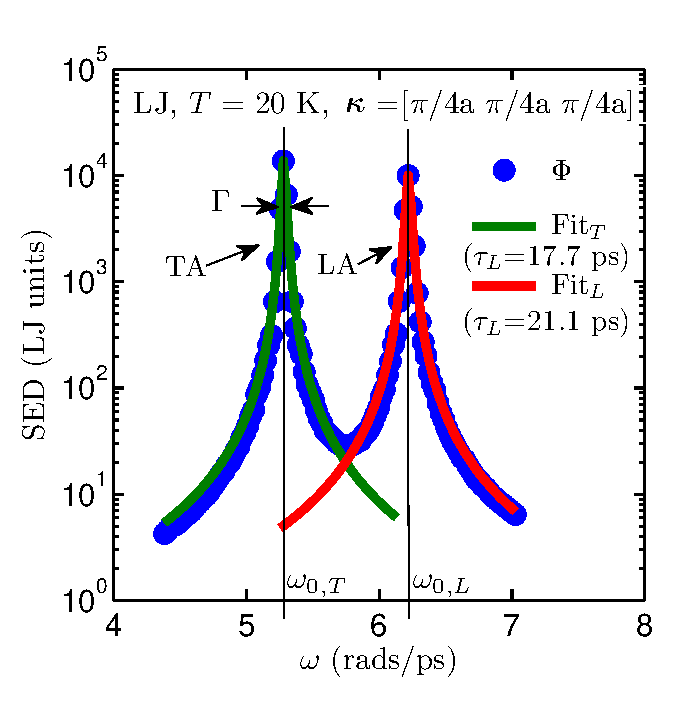
\includegraphics[angle=0,width=70.0mm]{figure1.eps}
\end{center}
\caption{\label{F:LJ_FIT_PEAK} The SED (using $\Phi$) for the first three polarizations at the wavevector $[\pi/4a,\pi/4a,\pi/4a]$ for LJ argon at a temperature of 20 K. There are two degenerate transverse acoustic (TA) polarizations and one longitudinal acoustic (LA) polarization. When fitting the SED, the different polarizations can be fit individually using single Lorentzian peaks or as a superposition of polarizations. Here the two peaks are fit individually with $\Phi$ plotted as a superposition and a single lifetime is predicted for each peak. The predicted lifetimes, which are inversely proportional to $\Gamma$ through Eq$.$ \eqref{E:lifetime}, are provided in the legend.}
\end{figure}



\subsection{\label{Subsection_Comp_Details_3}Thermal Conductivity}

Once the frequencies and lifetimes of all phonon modes in the first
Brillouin zone are obtained, the bulk thermal conductivity in direction
$\mathbf{n}$, $k_{\mathbf{n}}$, can be calculated from \cite{ziman2001}
\begin{equation}\label{E-size:k_bulk}\
\begin{split}
k_{\mathbf{n}}=&\sum_{\pmb{\kappa}} \sum_\nu c_{ph} \kv v^{2}_{g,\mathbf{n}} \kv \tau \kv.
\end{split}
\end{equation}
Here, $c_{ph}$ is the phonon volumetric specific heat and ${v}_{g,\mathbf{n}}$ is
the component of the group velocity vector in direction $\mathbf{n}$. Since the systems we consider are classical and obey Maxwell-Boltzmann statistics,\cite{mcquarrie2000} the
specific heat is $k_{\mathrm{B}}$ per mode in the harmonic limit, where $k_{\mathrm{B}}$ is the Boltzmann constant. As temperature increases, anharmonicity causes the mode specific heats to deviate from $k_{\mathrm{B}}$ \cite{mcgaughey2004c}. The effect is small for the systems and temperatures studied here. For LJ argon, the mode-averaged specific heat has been predicted to be $0.95k_{\mathrm{B}}$ per mode at a temperature of $40$ K and approaches $k_{\mathrm{B}}$ with decreasing temperature \cite{mcgaughey2004c}. For SW silicon at a temperature of $300$ K, the predicted mode-averaged specific heat is $1.01k_{\mathrm{B}}$ per mode \cite{goicochea2010}. For the CNT at $T=300$ K, we predict the mode-averaged specific heat to be $1.03k_{\mathrm{B}}$ per mode. For the three systems studied (argon, silicon, and CNT), we take the mode specific heats to be $k_{\mathrm{B}}$ per mode.  The group
velocity vector is the gradient of the dispersion curve (i.e., $\partial \omega / \partial \pmb{\kappa}$) and can be calculated from the frequencies and wavevectors using finite differences. In this work, the group velocities are calculated using the frequencies from quasi-harmonic lattice dynamics calculations because a smaller finite difference in wavevector can be used than what is available from the MD simulations (see Section \ref{Subsection_Comp_Details_1}).\footnote[2]{The anharmonic frequency shift affects the group velocity. McGaughey and Kaviany find that anharmonic and quasi-harmonic predictions of the group velocity differ for LJ Argon by less than one percent at a temperature of $50$ K, and the difference decreases with decreasing temperature.\cite{mcgaughey2004c} The anharmonic frequency shifts are on average a few percent for LJ argon at a temperature of $40$ K, and are less for the other temperatures and systems studied here.}

\subsection{\label{Subsection_Comp_Details_4}Computational Cost}

The computational cost of evaluating Eq. \eqref{Lorentzian_SED} is less than that for Eq$.$ \eqref{E:ave_T_w1} by a factor of $3b$, where $b$ is the number of atoms in the unit cell.  For bulk crystals, the number of atoms in the unit cell is typically small ($b<10$).  For the (8,8) CNT system, $b=32$ and evaluating $\Phi'$ is two orders of magnitude less expensive than evaluating $\Phi$.

To calculate the phonon lifetimes, the MD simulation time should be an order of magnitude longer than the longest phonon lifetime \cite{thomasthesis}.  If only the phonon frequencies are required, however, the location of the peaks in $\Phi$ and $\Phi'$ develop in a time on the order of the inverse of the phonon frequency, $1/\omega_0\kv$. For the systems studied here, this time can be two to five orders of magnitude less than the time needed to develop the lifetimes.

Fitting $\Phi'$ becomes challenging at higher temperatures, when the phonon linewidths broaden and become comparable to the spacing between mode frequencies. The cost of fitting $\Phi'$ can be reduced by fitting the peaks from all allowed wavevectors in the system simultaneously, but the error associated with this procedure is unknown \cite{shiomi2011a}. We find that a semi-automated procedure, whereby the fits are visualized, is necessary to ensure that all peaks are fit correctly.  While the computational cost of fitting $\Phi'$ is much smaller than the computational cost of calculating $\Phi'$, the semi-automated fitting procedure can be of similar time cost to the user. The cost of fitting $\Phi$ is much smaller because the different polarization peaks can be isolated and the fitting can be fully automated.

\section{\label{S:Section_Prop}Case Studies}

\subsection{\label{S:Subsection_prop_LJ}Lennard-Jones Argon}

We now use MD simulation to compare the SED, phonon properties, and thermal conductivity calculated for LJ argon using $\Phi$ and $\Phi'$. The MD simulations are performed using LAMMPS \cite{LAMMPS}. A truncated and shifted
potential cutoff scheme is used with a cutoff radius of 8.5 $\AA$. The quasi-harmonic phonon frequencies, eigenvectors, and group velocities are generated using GULP \cite{GULP}. We consider temperatures of 5, 20, and 40 K at zero-pressure with lattice constants of 5.278, 5.315, and 5.371 $\AA$. For LJ argon, Turney et al. found that lattice dynamics-based predictions of thermal conductivity (e.g., by anharmonic lattice dynamics or $\Phi$) start to diverge from MD-based predictions (e.g., from the direct or Green-Kubo methods) above half the melting temperature ($T_{\mathrm{melt}} \approx 80$ K) \cite{turney2009a}. In this paper, we limit the temperature to below half the melting temperature for the three systems studied (argon, silicon, and CNT).

The MD system consists of $N_1 \times N_2 \times N_3 = 8^3 = 512$ conventional cubic unit cells for a total of 2048 atoms ($b=4$ atoms). Using a 4.285 fs time step, the system is equilibrated for $2^{20}$ time steps before collecting data every $2^5$ time steps for an additional $2^{20}$ time steps in the $NVE$ ensemble (constant number of atoms, system volume, and total system energy) \cite{mcquarrie2000}. The sampling rate must be high enough to capture the highest phonon frequency in the system. The sampling rate and total run time are chosen in powers of two as a convenience in performing the fast Fourier transforms required to efficiently evaluate $\Phi$ and $\Phi'$. The same MD simulation data are used to calculate $\Phi$ and $\Phi'$.  Five simulations with different initial conditions are performed and the $\Phi$ and $\Phi'$ values are averaged before the peak fitting. $\Phi$ and $\Phi'$ are further averaged over degenerate wavevectors in the Brillouin zone, reducing the wavevectors to the first octant \cite{mcgaugheythesis}.

The SED ($\Phi$ and $\Phi'$) for the wavevector [$\pi/2a$,0,0] is presented in Fig$.$ \ref{F:PEAK_COMPARE} for all three temperatures (the edge of the Brillouin zone is at [$\pi/a$,0,0]).  For $\Phi$, the spectral curve is plotted as a superposition over the twelve phonon polarizations, with degeneracy reducing the number of peaks to seven.  Overall, $\Phi'$ does not equal the total phonon spectral energy density $\Phi$, but the major features are similar. We note that the linewidth (half of the inverse lifetime) defined in Eq$.$ \eqref{E:ave_T_w1} is independent of the Lorentzian peak magnitude. At all temperatures there are linewdith variations between the two spectral curves. The peak magnitudes become comparable for $\Phi$ and $\Phi'$ as the temperature increases.

\begin{figure}
\begin{center}
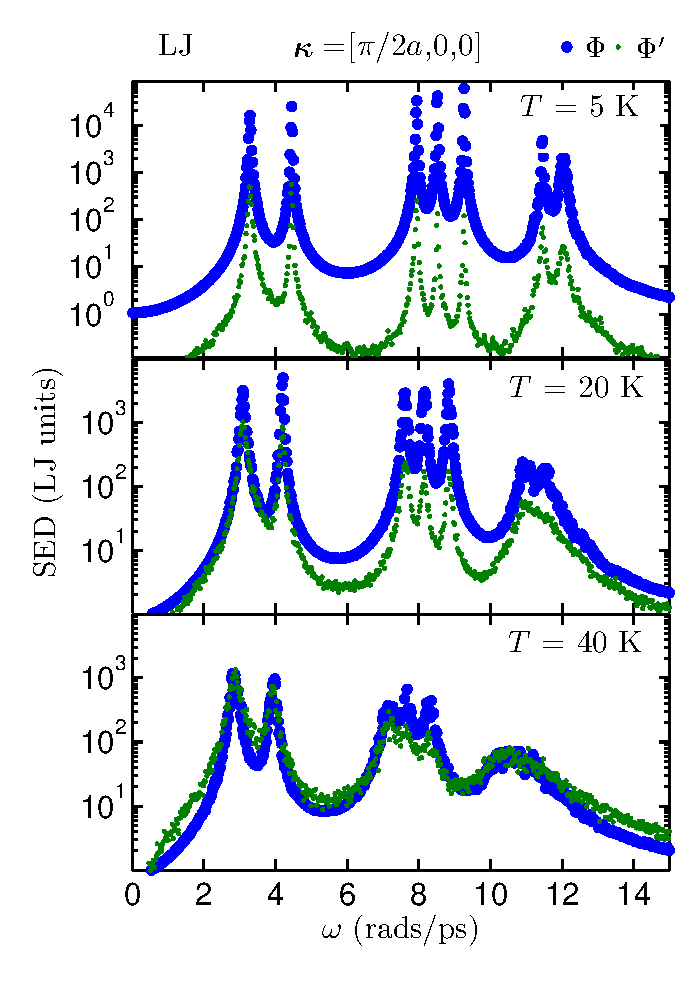
\includegraphics[angle=0,width=70.0mm]{figure2.eps}
\vspace*{0mm}
\end{center}
\caption{\label{F:PEAK_COMPARE} The phonon spectral energy density ($\Phi$) is plotted as larger blue circles.  The proposed alternative expression for the phonon spectral energy density ($\Phi'$) is plotted as smaller green points. The wavevector is ($\pi/2a$,0,0). Note that peak broadening at higher temperatures and frequencies above $10$ rads/ps can force peaks close in frequency for $\Phi'$ to be fit as a single Lorentzian function. $\Phi$ does not suffer from this issue since the broadened peaks can be fit individually.}
\end{figure}

The phonon frequencies and lifetimes extracted for all allowed wavevectors in the first Brillouin zone using $\Phi$ and $\Phi'$ at each of the three temperatures are compared on a mode-by-mode basis in Figs$.$ \ref{F:FREQ_LIFE_LJ}(a), \ref{F:FREQ_LIFE_LJ}(b), and \ref{F:FREQ_LIFE_LJ}(c). There, $\omega_0$, $\omega_0^{'}$, $\tau$, and $\tau^{'}$  refer to the mode properties predicted using $\Phi$ and $\Phi'$. The phonon frequencies agree well at all three temperatures, with increasing scatter at high temperatures and high frequencies.  This scatter is due to the high-frequency peak broadening seen in Fig$.$ \ref{F:PEAK_COMPARE} at $T = 40$ K, which can force peaks close in frequency for $\Phi'$ to be fit as a single Lorentzian function. The frequencies predicted by $\Phi$ and $\Phi'$ include the effects of anharmonicity, which increase the frequencies compared to the quasi-harmonic predictions \cite{mcgaughey2004c,turney2009a}. The agreement between the frequencies predicted from $\Phi$ and $\Phi'$ is explained in \ref{Appendix_B}.

The lifetimes show large scatter between $\Phi$ and $\Phi'$ on a mode-by-mode basis, with increasing scatter at high temperature that shows no systematic difference. The scatter at high frequencies is in part due to the peak broadening seen in Fig$.$ \ref{F:PEAK_COMPARE}, which can force peaks close in frequency for $\Phi'$ to be fit as a single Lorentzian function with a single lifetime. The broadening does not affect fitting at low frequencies, where the linewidths are much smaller than the peak spacings. There, any scatter comes solely from the difference between $\Phi$ and $\Phi'$.

\begin{figure}
\begin{center}

\subfigure{
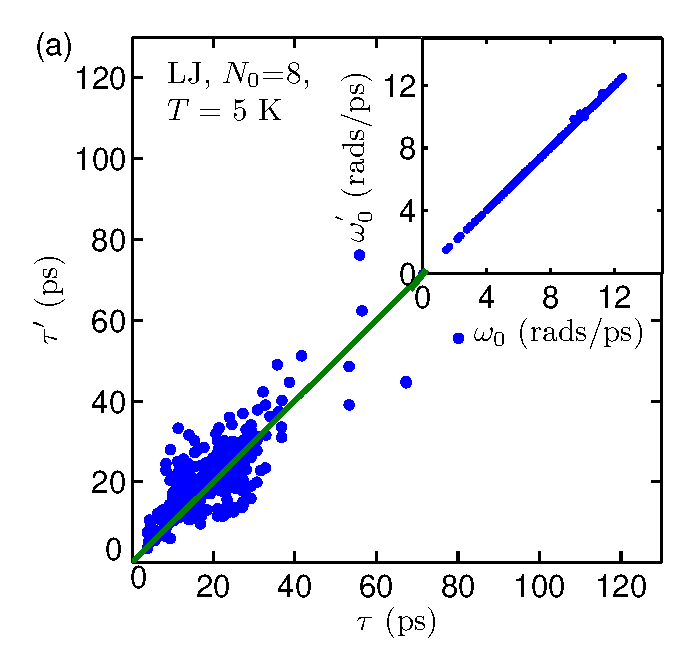
\includegraphics[angle=0,width=70.0mm]{figure3_a.eps}
}

\subfigure{
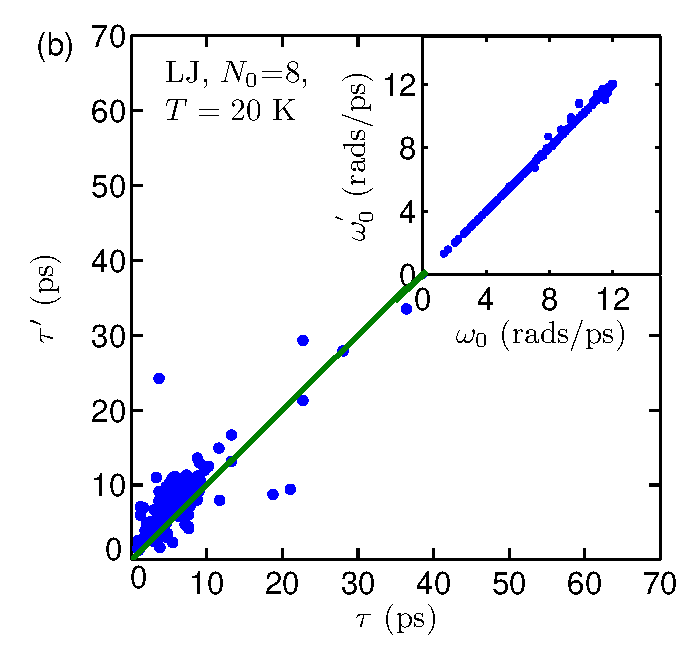
\includegraphics[angle=0,width=70.0mm]{figure3_b.eps}
}

\subfigure{
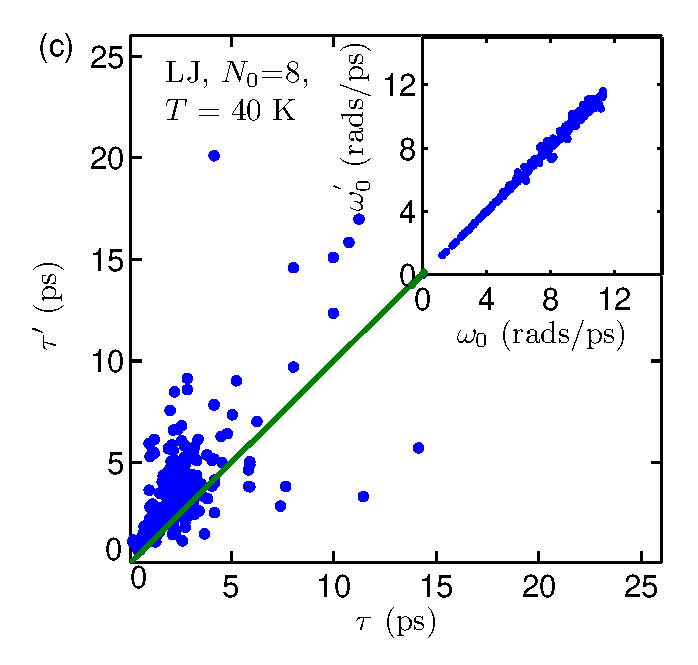
\includegraphics[angle=0,width=70.0mm]{figure3_c.eps}
}

\end{center}
\caption{\label{F:FREQ_LIFE_LJ} Comparison of the phonon frequencies and lifetimes predicted using $\Phi$ ($\omega$ and $\tau$) and $\Phi'$ ($\omega^{'}$ and $\tau^{'}$) for LJ argon at temperatures of (a) 5 K, (b) 20 K, and (c) 40 K. The phonon frequencies agree well at all three temperatures, while the phonon lifetimes show large scatter.}
\end{figure}



The phonon properties are then used to predict thermal conductivity using Eq$.$ \eqref{E-size:k_bulk}. The results are presented in Table \ref{T:cond_table}. The bulk thermal conductivities provided in Table \ref{T:cond_table} are predicted using the finite simulation-size scaling procedure discussed in \ref{Appendix_C}. The bulk thermal conductivities predicted from $\Phi'$ are smaller and outside the uncertainty for those predicted from $\Phi$ for temperatures of $5$ and $20$ K. While the bulk thermal conductivities at a temperature of $40$ K agree within their uncertainties, the predicted mode-by-mode lifetimes show large scatter [Fig$.$ \ref{F:FREQ_LIFE_LJ}(c)] and the agreement should be regarded as coincidental.

The disagreement between $\Phi$ and $\Phi'$ in thermal conductivity comes directly from the differences in the phonon lifetimes. All other properties (frequencies, group velocities, specific heats) are nearly or exactly the same for the two calculations. The bulk thermal conductivities predicted from $\Phi$ and $\Phi'$ are also compared to predictions from the Green-Kubo method\cite{mcquarrie2000} in Table \ref{T:cond_table}. For $N_1=N_2=N_3=8$, the thermal conductivity predicted by the Green-Kubo method is converged with respect to the simulation size \cite{mcgaughey2004c}. The same MD data used to calculate $\Phi$ and $\Phi'$ is used for the Green-Kubo predictions. For all three temperatures, there is good agreement between the thermal conductivity predictions using $\Phi$ and Green-Kubo. For temperatures of $20$ and $40$ K, there is good agreement between the predictions from $\Phi$, Green-Kubo, and previous reports using non-equilibrium MD, anharmonic lattice dynamics, and time-domain $\Phi$ \cite{turney2009a}.

\begin{center}
\begin{table}
\caption{\label{T:cond_table}Thermal conductivity values in W/m-K predicted using $\Phi$, $\Phi'$, and the Green-Kubo methods.  The predictions for $\Phi$ and Green-Kubo for the LJ system are in good agreement with those from other atomistic simulation methods\cite{turney2009a} while those from $\Phi'$ differ and show no systematic behavior. The uncertainties in the predicted thermal conductivities for $\Phi$ and $\Phi'$ come predominantly from the finite simulation-size scaling procedure (see \ref{Appendix_C}).}
\begin{ruledtabular}
\begin{tabular}{llllll}
     &                             &         &      &   \\
$T$ (K)&Green-Kubo \ &$\Phi$ &$\Phi'$\\
\hline
LJ (bulk)\\
5&8.0 $\pm$ 0.30 &7.9 $\pm$ 0.42 &5.8 $\pm$ 0.31 \\
20&1.3 $\pm$ 0.15 &1.2 $\pm$ 0.07 &1.0 $\pm$ 0.10 \\
40&0.45 $\pm$ 0.07 &0.47 $\pm$ 0.03 &0.49 $\pm$ 0.05 \\
\hline
SW ($N_1=N_2=N_3=6$) \\
300& &322 $\pm$ 16 &396 $\pm$ 38 \\
\hline
CNT ($N_1=N_2=1, N_3=50$) \\
300& &428 $\pm$ 21 &398 $\pm$ 40 \\
\end{tabular}
\end{ruledtabular}
\end{table}
\end{center}

\vspace*{70mm}

\subsection{\label{S:Subsection_prop_SW}Stillinger-Weber Silicon}

We next compare the phonon properties and thermal conductivity predicted from $\Phi$ and $\Phi'$ for SW silicon \cite{stillinger1985} at a temperature of $300$ K and zero pressure with a lattice constant of 5.437 $\AA$. The SW system is stiffer (larger phonon group velocities, frequencies, and lifetimes) than LJ argon and is an additional test to determine if there is a systematic error in the predictions from $\Phi'$. The MD simulations are performed using LAMMPS \cite{LAMMPS}. The MD system consists
of $N_1 \times N_2 \times N_3 = 6^3 = 216$ conventional unit cells for a total of 1728 atoms ($b=8$ atoms). The phonon frequencies, eigenvectors, and group velocities are generated using GULP \cite{GULP}.

Using a 0.5 fs timestep, the system is equilibrated for $2^{20}$ time steps before collecting data every $2^5$ time step for $2^{22}$ time steps in the $NVE$ ensemble \cite{mcquarrie2000}. As with the LJ system, the sampling rate is determined by the highest phonon frequency in the system. Five simulations with different initial conditions are performed and the $\Phi$ and $\Phi'$ values are averaged before the peak fitting. $\Phi$ and $\Phi'$ are further averaged over degenerate wavevectors in the Brillouin zone, reducing the wavevectors to the first octant \cite{mcgaugheythesis}.

The extracted phonon frequencies and lifetimes are plotted in Fig$.$ \ref{F:FREQ_LIFE_Si}. As with the LJ system, the phonon frequencies are predicted accurately by $\Phi'$ but the lifetimes show large scatter on a mode-by-mode basis. For the system size studied, $\Phi'$ predicts a larger thermal conductivity than $\Phi$ outside the prediction uncertainties, in contrast to the LJ system (see Table \ref{T:cond_table} and \ref{Appendix_C}). The disagreement in thermal conductivity comes directly from the predicted phonon lifetimes.

\begin{figure}
\begin{center}
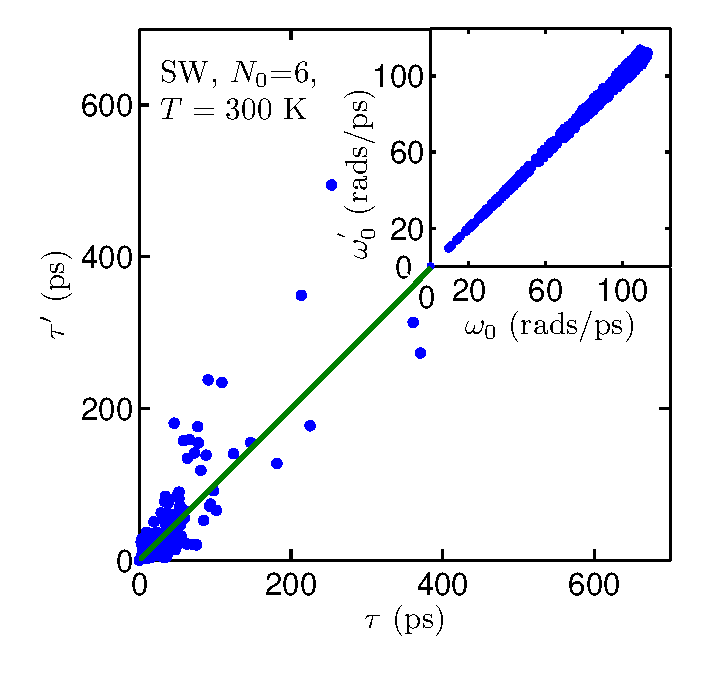
\includegraphics[angle=0,width=70.0mm]{figure4.eps}
\vspace*{0mm}
\end{center}
\caption{\label{F:FREQ_LIFE_Si} Comparison of the phonon frequencies and lifetimes predicted using $\Phi$ ($\omega$ and $\tau$) and  $\Phi'$ ($\omega'$ and $\tau'$) for SW silicon. The phonon frequencies agree well, while the phonon lifetimes show large scatter.}
\end{figure}

%\vspace*{60mm}

\subsection{\label{S:Subsection_prop_CNT}Carbon Nanotube}

Finally, we compare the phonon properties and thermal conductivities predicted by $\Phi$ and $\Phi'$ for an (8,8) CNT (diameter of 1.10-nm and length of 12.3 nm) at a temperature of $300$ K and zero pressure \cite{thomas2010c}. The interactions in the CNT system are modeled using the REBO potential without the four-body interaction term \cite{brenner2002}. The MD simulations are performed using an in-house code. The MD system consists of 1600 atoms (32 atoms/unit cell). The phonon frequencies, eigenvectors, and group velocities are generated using an in-house code. The purpose of simulating this system is to check the results of Thomas et al.\cite{thomas2010c} (who used $\Phi'$ and non-equilibrium MD), and to compare the predictions of $\Phi'$ and $\Phi$.

Using a 1.0 fs timestep, the system is equilibrated for $2^{20}$ time steps before collecting data every $2^3$ time step for $2^{22}$ time steps in the $NVE$ ensemble \cite{mcquarrie2000}. As with the LJ and SW systems, the sampling rate is determined by the highest phonon frequency in the system. Five simulations with different initial conditions are performed and the $\Phi$ and $\Phi'$ values are averaged before the peak fitting. Since the Brillouin zone of the CNT is one-dimensional, $\Phi$ and $\Phi'$ are further averaged over directionally-degenerate wavevectors.

The phonon frequencies and lifetimes for the allowed wavevectors in the one-dimensional Brillouin zone of the CNT are shown in Fig. \ref{F:FREQ_LIFE_CNT}. Like the LJ and SW silicon systems, the phonon frequencies can be predicted accurately by $\Phi'$, but the lifetimes show large scatter. The estimated thermal conductivity of the CNT predicted using $\Phi'$ is in agreement with the results of Thomas et al.\cite{thomas2010c} The thermal conductivity predicted by $\Phi'$ is less than that predicted by $\Phi$, but not outside their uncertainties.

\begin{figure}
\begin{center}
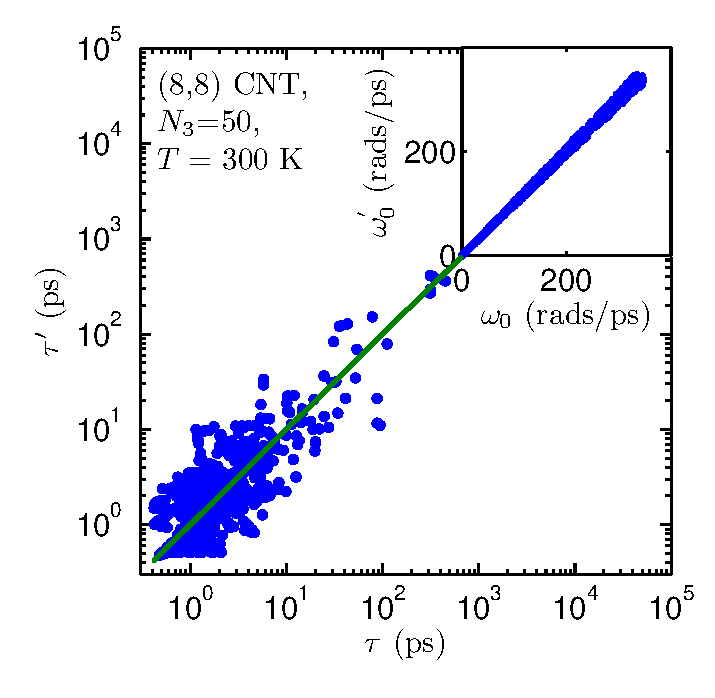
\includegraphics[angle=0,width=70.0mm]{figure5.eps}
\vspace*{0mm}
\end{center}
\caption{\label{F:FREQ_LIFE_CNT} Comparison of the phonon frequencies and lifetimes predicted using $\Phi$ ($\omega,\tau$) and $\Phi'$ ($\omega',\tau'$) for a (8,8) CNT modeled using the REBO potential. The phonon frequencies agree well, while the phonon lifetimes show large scatter.}
\end{figure}

\vspace*{0mm}

\section{\label{Section_Conclusions}Summary}

We derived the correct phonon SED, $\Phi$, and its relation to the phonon frequencies and lifetimes by starting from the normal mode coordinates. We then presented an alternative formulation to the phonon spectral energy density, $\Phi'$, which does not require the phonon mode eigenvectors.  Because $\Phi'$ does not contain the eigenvectors, this alternative formulation does not represent the phonon spectral energy density, but does contain information about the phonon dispersion as the temperature approaches $0$ K (see \ref{Appendix_B}).

We then calculated the phonon SED for LJ argon, SW silicon, and a CNT modeled with the REBO potential using $\Phi$ and $\Phi'$. The phonon frequencies and
lifetimes predicted from $\Phi$ and $\Phi'$ are shown in Figs$.$ \ref{F:FREQ_LIFE_LJ}, \ref{F:FREQ_LIFE_Si} and \ref{F:FREQ_LIFE_CNT}. The
frequencies are in good agreement between the two SED methods, while the lifetimes show large scatter.

The phonon SED $\Phi$ is well-defined theoretically, while $\Phi'$ does not properly map to the phonon energies since it is missing the phonon mode eigenvector. We deduce that this is the reason $\Phi'$ does not accurately predict the phonon lifetimes. It is surprising, however, how close the predicted thermal conductivities can be using $\Phi$ and $\Phi'$ (LJ at $T=40$ K and the CNT results).

Still, the most important predictions are the mode-by-mode phonon properties. Of particular importance are the lifetimes, which are the key input for Boltzmann transport equation-based models \cite{mcgaughey2011a}. Thus, we do not recommend $\Phi'$ for predicting phonon lifetimes or thermal conductivity.  Any agreement in thermal conductivity predictions between atomistic studies\cite{thomas2010c} and experiment\cite{dekoker2009,qiu2011} must be regarded as coincidental, and the phonon lifetime reductions predicted for systems with additional scattering methods \cite{thomas2010c,shiomi2011a} should only be interpreted qualitatively.

\ack
This work is supported by AFOSR award FA95501010098. We thank John A. Thomas (Johns Hopkins University Applied Physics Laboratory) for helpful discussions.
%\end{acknowledgments}

\vspace*{190mm}
\appendix
\section{\label{Appendix_A}Derivation of Phonon Spectral Energy Density, $\Phi$}

We start from Eq$.$ \eqref{E:qdot_HLD} and follow the formulation of anharmonic lattice dynamics theory \cite{maradudin1974,wallace1972,dove1993,srivastava1990}. In an anharmonic system, the phonon populations fluctuate about the
equilibrium distribution function \cite{wallace1972}. The phonon mode coordinate for the mode described by ($\pmb{\kappa},\nu$) and its time
derivative can be written as
\begin{equation}\label{A:E:q_A}
\begin{split}
q\kvt=&q_{SS}\kvt+q_{T}\kvt
\end{split}
\end{equation}
and
\begin{equation}\label{A:E:qdot_A}
\begin{split}
\dot{q}\kvt=& \dot{q}_{SS}\kvt+\dot{q}_{T}\kvt.
\end{split}
\end{equation}
The steady-state ($SS$) and transient ($T$) parts and their time derivatives are given by
\begin{equation}\label{A:E:q_A_SS}
\begin{split}
q_{SS}\kvt=& C_1\kv\exp[i\omega_0\kv t]
\\& +C_2\kv\exp[-i\omega_0\kv t],
\end{split}
\end{equation}
\begin{equation}\label{A:E:q_A_T}
\begin{split}
q_{T}\kvt=& \EXP{-\Gamma\kv |t|}\lbrace C_3\kv\EXP{i\omega_0\kv t}
\\ &-C_4\kv\EXP{-i\omega_0\kv t } \rbrace,
\end{split}
\end{equation}
\begin{equation}\label{A:E:qdot_A_SS}
\begin{split}
\dot{q}_{SS}\kvt=& i\omega_0\left\{C_1\kv\exp[i\omega_0\kv t]-C_2\kv\exp[-i\omega_0\kv t]\right\} ,
\end{split}
\end{equation}
and
\begin{equation}\label{E:qdot_A_T}
\begin{split}
\dot{q}_{T}\kvt=& \EXP{-\Gamma\kv |t|}\left\{C_3\kv\left[i\omega_0\kv-\Gamma\kv\right]\EXP{i\omega_0\kv t}\right. \\
& \left.-C_4\kv\left[i\omega_0\kv+\Gamma\kv\right]\EXP{-i\omega_0\kv t}\; \right\},
\end{split}
\end{equation}
where the $C$s are constants and $\omega_0\kv$ and $\Gamma\kv$ are the phonon
mode frequency and linewidth.  The transient part
describes the creation of an excess in the population of a phonon mode for
$t<0$ and its decay back to equilibrium for $t>0$.

Phonon population fluctuations are commonly modeled using the excitation and decay of
a single phonon mode (i.e., the single mode relaxation time approximation). In a real system, there will be multiple phonons in
each mode that simultaneously grow or decay with time.  Thus, dealing only
with $\dot{q}$, we let
\begin{equation}\label{A:E:qdot_A_kvbat}
\begin{split}
\dot{q}\kvt =& \sum_j i\EXP{-\Gamma\kv |t-t_j|}\times \\
& \lbrace A_j\kv\left[\omega_0\kv+i\Gamma\kv\right]\EXP{i\omega_0\kv (t-t_j)} \\
& -B_j\kv \left[\omega_0\kv-i\Gamma\kv\right]\EXP{-i\omega_0\kv (t-t_j) } \; \rbrace,
\end{split}
\end{equation}
where many phonons in each mode, indexed by $j$, are simultaneously being
created and destroyed.  The phonons grow for $t<t_j$, decay for $t>t_j$,
and $A_j$ and $B_j$ are constants.  We are  not concerned with the values of
$t_j$, $A_j$, and $B_j$, though they should satisfy the long-time average
$\langle\dot{q}^*\kvt\dot{q}\kvt\rangle = \langle\dot{q}_{SS}^*\kvt\dot{q}_{SS}\kvt\rangle$.

The expectation value of the kinetic energy of the normal mode in the time domain is
\begin{equation}\label{A:E:ave_T_t}
\begin{split}
\langle T\kv \rangle=&\frac{1}{2}\lim_{\tau_0\rightarrow\infty}\frac{1}{\tau_0}\int_{0}^{\tau_0}\dot{q}^*\kvt\dot{q}\kvt dt.
\end{split}
\end{equation}
The expectation value of the kinetic energy of the normal mode can be transformed from the time domain to the
frequency domain by Parseval's theorem,\cite{rudin1987} giving
\begin{equation}\label{A:E:ave_T_w1}
\begin{split}
T\kvw=&\lim_{\tau_0\rightarrow\infty}\frac{1}{2\tau_0}\left|\frac{1}{\sqrt{2\pi}}\int_{0}^{\tau_0}\dot{q}\kvt\exp(-i\omega t)dt\right|^2.
\end{split}
\end{equation}
By substituting Eq$.$ \eqref{A:E:qdot_A_kvbat} into Eq$.$ \eqref{A:E:ave_T_w1} and performing the time integration we find
\begin{equation}\label{A:E:ave_T_w_int}
\begin{split}
T\kvw = \frac{1}{16\pi\tau_0}\left|\sum_j\EXP{-i\omega t_j} \left\{A_j\kv\frac{\omega_0\kv+i\Gamma\kv}{\omega_0\kv-\omega+i\Gamma\kv}\right.\right.\\
\left.\left.+B_j\kv\frac{\omega_0\kv-i\Gamma\kv}{\omega_0\kv+\omega-i\Gamma\kv}\right\}\right|^2.
\end{split}
\end{equation}
We are primarily interested in values of $\omega$ where $\omega\approx\omega_0$ when $\Gamma<<\omega_0$ (this condition is met for the three systems studied here).  When $\omega\approx\omega_0$, the term involving $A_j$ becomes large and the term involving $B_j$ can be neglected (alternatively, we could ignore the term involving $A_j$ when $\omega\approx-\omega_0$).  Hence, we find
\begin{equation}\label{A:E:ave_T_w_approx}
\begin{split}
T\kvw=\frac{1}{16\pi\tau_0}\sum_j\sum_{j'}\cos\left[\omega (t_{j'}-t_j)\right]A_j\kv A_{j'}\kv\\
\times\frac{\omega_0^2\kv+\Gamma^2\kv}{\Gamma\kv}\frac{\Gamma\kv}{[\omega_0\kv-\omega]^2+\Gamma^2\kv}.
\end{split}
\end{equation}
We arrive at the expression for the phonon spectral energy density for the wavevector $\pmb{\kappa}$ by summing Eq$.$ \eqref{A:E:ave_T_w_approx} over the different polarizations $\nu$,
\begin{equation}\label{A:E:Lorentzian_NMD}
\begin{split}
\Phi(\pmb{\kappa},\omega) = 2\sum_{\nu}^{3n} T\kvw=\sum_{\nu}^{3n}C_0\kv\frac{\Gamma\kv/\pi}{[\omega_0\kv-\omega]^2+\Gamma^2\kv},
\end{split}
\end{equation}
where the factor of two comes from equipartition of kinetic and potential energy (valid for a harmonic classical system, see Section \ref{Subsection_Comp_Details_3}), and
\begin{equation}\label{A:E:C_0}
\begin{split}
C_0\kv = \sum_j\sum_{j'}\cos\left[\omega (t_{j'}-t_j)\right]A_j\kv A_{j'}\kv\frac{\omega_0^2\kv+\Gamma^2\kv}{8\tau_0\Gamma\kv}.
\end{split}
\end{equation}
Thus, the phonon spectral energy density $\Phi(\pmb{\kappa},\omega)$ is a superposition of $3n$ Lorentzian
functions with centers at $\omega_0\kv$ (one for each polarization) with a linewidth (half-width at half-maximum) of
$\Gamma\kv$. $\Phi$ is a spectral energy density since its integral over all wavevectors and frequencies is the total crystal energy, i.e., the Hamiltonian is
\begin{equation}\label{A:E:equipartition}
\begin{split}
H=\int\limits_{V_{BZ}} \int_{0}^{\infty}\Phi(\pmb{\kappa},\omega)d\omega d\pmb{\kappa},
\end{split}
\end{equation}
where $V_{BZ}$ is the volume of the first Brillouin zone.  Like the frequency broadening, there is also a broadening of the SED in wavevector \cite{turneythesis}. For a finite sampling of the first Brillouin zone, the Hamiltonian can be approximated by
\begin{equation}\label{A:E:equipartition}
\begin{split}
H \approx 2\sum_{\pmb{\kappa},\nu}^{N,3n}\langle T\kvt\rangle = \sum_{\pmb{\kappa}}^N \int_{0}^{\infty}\Phi(\omega,\pmb{\kappa})d\omega.
\end{split}
\end{equation}

\section{\label{Appendix_B}Interpretation of $\Phi'$}

As demonstrated in Section \ref{S:Subsection_prop_LJ}, $\Phi'$ is not the phonon spectral energy density, $\Phi$, defined by Eq$.$ \eqref{E:ave_T_w1}. Our findings and those of others,\cite{maruyama2003,dekoker2009,thomas2010c,qiu2011,shiomi2011a} however, suggest that $\Phi'$ does contain accurate information about the phonon frequencies.  Under the harmonic approximation, the phonons are non-interacting and have no transient response beyond a harmonic oscillation (see \ref{Appendix_A} Eq$.$ \eqref{A:E:qdot_A} and \eqref{E:qdot_A_T}),
\begin{equation}\label{E:qdot_A_SS}
\begin{split}
\dot{q}\kvt =& \dot{q}_{SS}\kvt  \\
=& i\omega_0\kv\left\{C_1\kv\exp[i\omega_0\kv t]-C_2\kv\exp[-i\omega_0\kv t]\right\}.
 \end{split}
\end{equation}
Inserting Eq$.$ \eqref{E:qdot_A_SS} into the right hand side of Eq$.$ \eqref{SED} gives
\begin{equation}\label{Delta_SED}
\begin{split}
\sum_\alpha^3 \sum_b^n m_b \left| \sum_l^N  \int_{-\infty}^{\infty} \dot{u}_{\alpha}\lbt \EXP{i\pmb{\kappa}\cdot\mathbf{r}_0\ab{l}{0}-i\omega t} dt \right|^2 =& \\
\sum_\alpha^3 \sum_b^n\left| \frac{m_b^{3/2}}{\sqrt{N}} \sum_l^N \sum_{\nu}^{3n}  D\kvba \EXP{i\pmb{\kappa}\cdot\mathbf{r}_0\ab{l}{0}} \delta[ \omega_0\kv - \omega] \right|^2 ,
 \end{split}
\end{equation}
where $D\kvba = i\sqrt{2\pi} \omega_0\kv C_1\kv e^*\kvba$, $\delta$ is the Dirac function, and values of $\omega \le 0$ are ignored. Thus, at zero temperature Eq$.$ \eqref{Lorentzian_SED} is a superposition of Dirac functions at the phonon frequencies $\omega_0\kv$.

\section{\label{Appendix_C}Finite Simulation-Size Scaling for Thermal Conductivity}

For the LJ argon system studied in Section \ref{S:Subsection_prop_LJ}, a finite simulation-size scaling procedure\cite{turney2009a,He2011} is used to compare the thermal conductivity predictions from $\Phi$ and $\Phi'$ to those from the Green-Kubo method. The scaling procedure is demonstrated in Fig$.$ \ref{F:LJ_COND}.  The thermal conductivity is predicted from $\Phi$ or $\Phi'$ and MD simulations with $N_0 = 4,6,8,$ and $10$. The bulk conductivity, $k_{\infty}$, is then estimated by fitting the data to
\begin{equation}\label{k_size}
\begin{split}
1/k = 1/k_{\infty} + A/N_0,
 \end{split}
\end{equation}
where $A$ is a constant. This procedure is necessary because the first Brillouin zone is only sampled at a finite number of points for a finite simulation size, with no contribution from the volume at its center. To predict a bulk thermal conductivity, it is important to sample points near the Brillouin zone center, where the modes can have large lifetimes and group velocities \cite{turney2009a,sellan2010b}. As with the extrapolated bulk thermal conductivities at temperatures of $5$ and $20$ K (see Table \ref{T:cond_table}), the predicted thermal conductivities at each system size ($N_0=4,6,8,$ and $10$) are systematically smaller and outside the prediction uncertainties for $\Phi'$ compared to $\Phi$.

%This method has been validated for non-equilibrium MD simulations \cite{sellan2010a}, but has not been validated for equilibrium MD.
\begin{figure}
\begin{center}
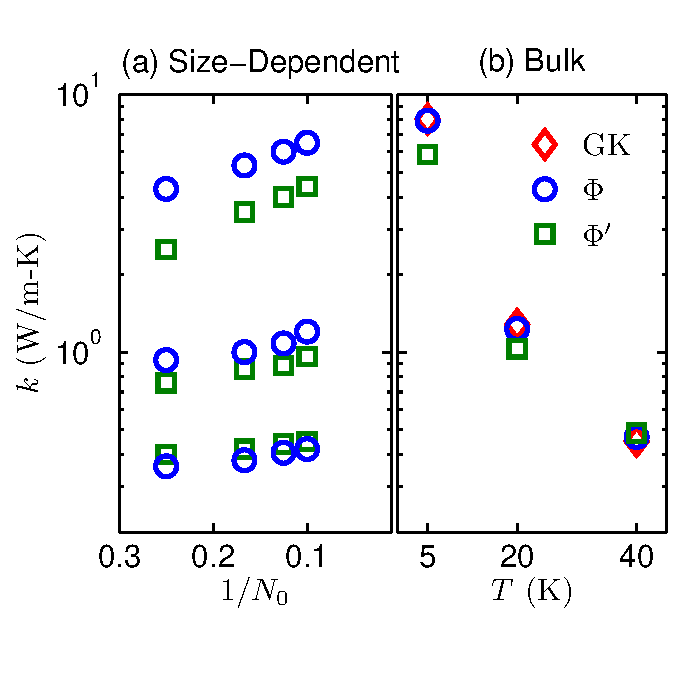
\includegraphics[angle=0,width=70.0mm]{figure6.eps}
\caption{\label{F:LJ_COND} Thermal conductivity predictions for LJ argon calculated using phonon lifetimes predicted by $\Phi$ and $\Phi'$. (a) The finite simulation-size scaling extrapolation \cite{turney2009a,He2011} is used to compare the results to bulk predictions made using the Green-Kubo method. (b) The bulk results for $\Phi$ and Green-Kubo are in good agreement temperatures of $20$ and $40$ K with those of other atomistic simulation methods,\cite{turney2009a} while those from $\Phi'$ differ (see Table \ref{T:cond_table}).}
\end{center}
\end{figure}

\setcounter{section}{1}

\vspace*{100mm}


% Create the reference section using BibTeX:
\bibliographystyle{unsrt}

\bibliography{references}

%\end{multicols}

\end{document}
%
% ****** End of file ******
